\section{Experimental Evaluation}
\label{sec:experimentalevaluation}
We test our models by the ability to forecast proton flux at two horizons: 30 minutes $(t+6)$ and 60 min $(t+12)$. the second task is forecasting the occurrence of SEP events (protons intensity exceeding a threshold) 30 and 60 minutes ahead.

\subsection{Evaluation of SEP Time-Intensity Profile Prediction}
\subsubsection{Evaluation Criteria}
\cite{torres2025machine} uses two grading criteria for their models: lag and MAE.
The intensity models are graded using mean absolute error (MAE). this calculates the absolute difference between the actual and predicted values at each timestamps. We do not care about background noise portion of our so we only evaluate when a rise in proton flux occurs to the peak (onset to peak).

\begin{align}
    MAE = \frac{1}{n}\sum |x_{\text{model}}-x_{\text{obs}}|
\end{align}

Lag is another graded feature we are interested in. We want to know whether predictions are on time or too late. we shift our predictions between the onset and peak of each event and test to align with the targets and measuring MAE at each shift. The shift with the lowest MAE is considered the lag.

A third prediction efficiency metric is used as a comparison as well. For a discrete time series as

\begin{align}
  PE = 1 - \frac{\langle (x_{\text{model}} - x_{\text{obs}})^2\rangle}{\sigma^2_{\text{obs}}}  
\end{align}

with $\langle . \rangle$ denoting arithmetic mean, $x_{\text{obs}}$ the observation, $x_{\text{mod}}$ the modeled signal, and $\sigma_{\text{obs}}^2$ as the variance in the observed signal. PE indicated perfect model performance and PE = 0 indicated performance comparable to predicting the arithmetic mean of the observed signal. PE can reach unlimited negative values. \cite{Rastatter2011PE}

An F1 score evaluates the performance of our forecasting model. The score is calculated by arithmetic operations of the number of true positive, false positives, and false negatives the solve into the recall \eqref{recall} and precision \eqref{precision}. the recall and precision values are then used to calculate our final F1 score \eqref{F1}:
\begin{equation}
    \label{recall}
    \text{recall} = \frac{TP}{TP + FN} 
\end{equation}
\begin{equation}
    \label{precision}
    \text{precision} = \frac{TP}{TP+FP}
\end{equation}
\begin{equation}
    \label{F1}
    \text{F1} = \frac{2 \times \text{precision} \times \text{recall}}{\text{precision} + \text{recall}}
\end{equation}.
\subsubsection{Learning and Evaluation Procedures}
We do ten randomized 80/20 splits of  our raw particle intensity data into training and test sets chronologically respectively. Each train/test split runs 10 models with each seed totaling 100 models for one forecasting time \cite{pastore2021extrapolating} . One of the train/test split is the original chronological split that Torres uses where there is 21 SEP identified events in the training set and 18 SEP events in the test set. \citeA[Table 1]{torres2025machine}. 

To properly compare our transformer model with RNN and NN models we train the transformer to minimizes loss by the mean square error (MSE) in log space between the target proton intensity and the predicted proton intensity. The output will also be in natural logarithm space \cite{torres2025machine}.

To match the RNN and NN, weights are updated using Adam optimizer and we converge if the loss function does not change by more the $10^{-4}$ over 20 iterations. We train five separate models at different seeds $(1-5)$ and average and standard deviation of MAE and lag \cite{torres2025machine}.



\subsubsection{Baseline Methods Used for Comparison}
\cite{torres2025machine} uses a persistent model as a baseline for their RNN and NN models. its a simple baseline method in which the predicted proton flux value is the current proton flux value, which is equivalent to now cast. \cite{posner2007forecasting} matrix will be compared to as well across the same metrics.

A linear regression model implemented from pythons SkLearn library will also be used as a baseline for our transformer

The baseline models are deterministic so we will only report a single run

\subsubsection{Results}

We compare the performance of our models to the different methods offered by Torres for t+6 and t+12 in Figure \ref{fig:mae_lag_comparison}. For both t+6 and t+12 we see similar behavior. All models of different architecture (Rope, Sinusoidal, Zero Init) tend to outperform Torres's RNN and NN for MAE at both $t+6$ and $t+12$ Neural network models have more fluctuation in their predictions which can yield larger vertical gaps, particularity when the proton flux is relatively flat or slow rising \cite{torres2025machine}.

Lag, however, tends to measure larger. Torres explained their lag problem underperformed \cite{posner2007forecasting} forecasting matrix as the method over predicts proton intensity. Reducing the lag in the forecasting was hoped to be solved by a transformer. 


\begin{figure}[!htbp]
    \centering
    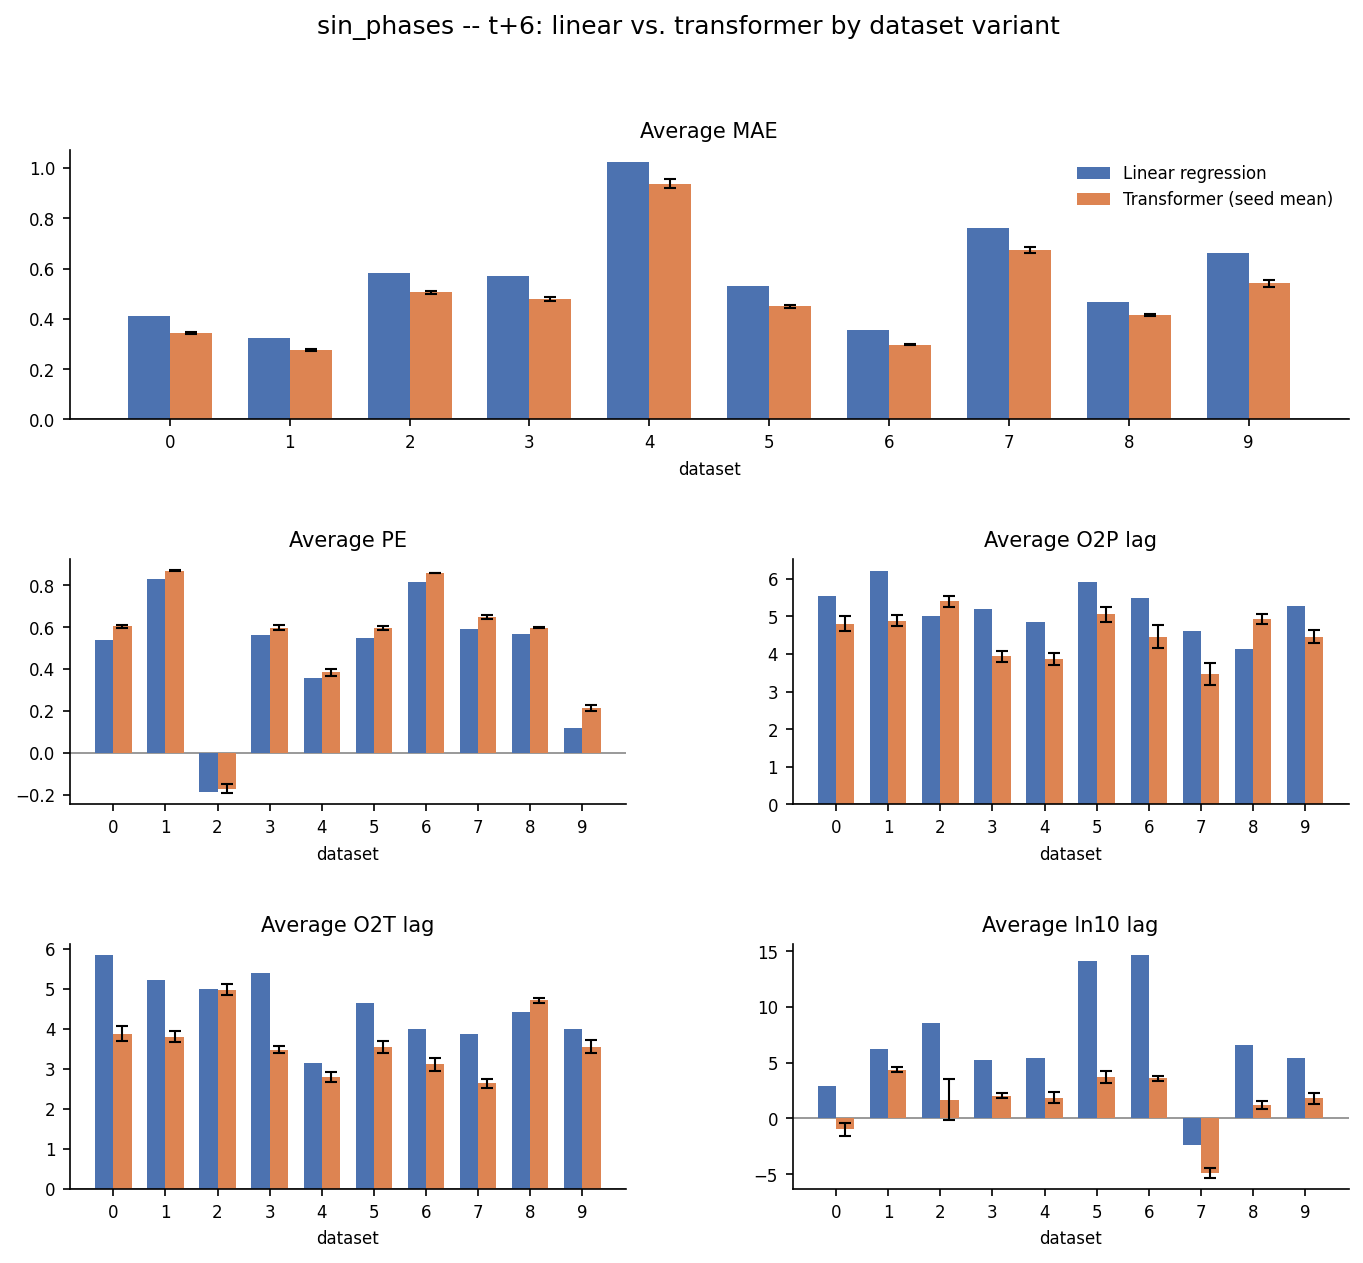
\includegraphics[width=0.7\textwidth]{plots/sin_phases_t6_linear_vs_transformer.png}
    \caption{This image is from real results from my cross validation split of 10 datasets but only for my sin encoded transformer. incomplete but wanted to show this here for now.}
    \label{fig:sinusoidal_t6_comparison}
\end{figure}

\begin{figure}[H]
    \centering % Centers the image
    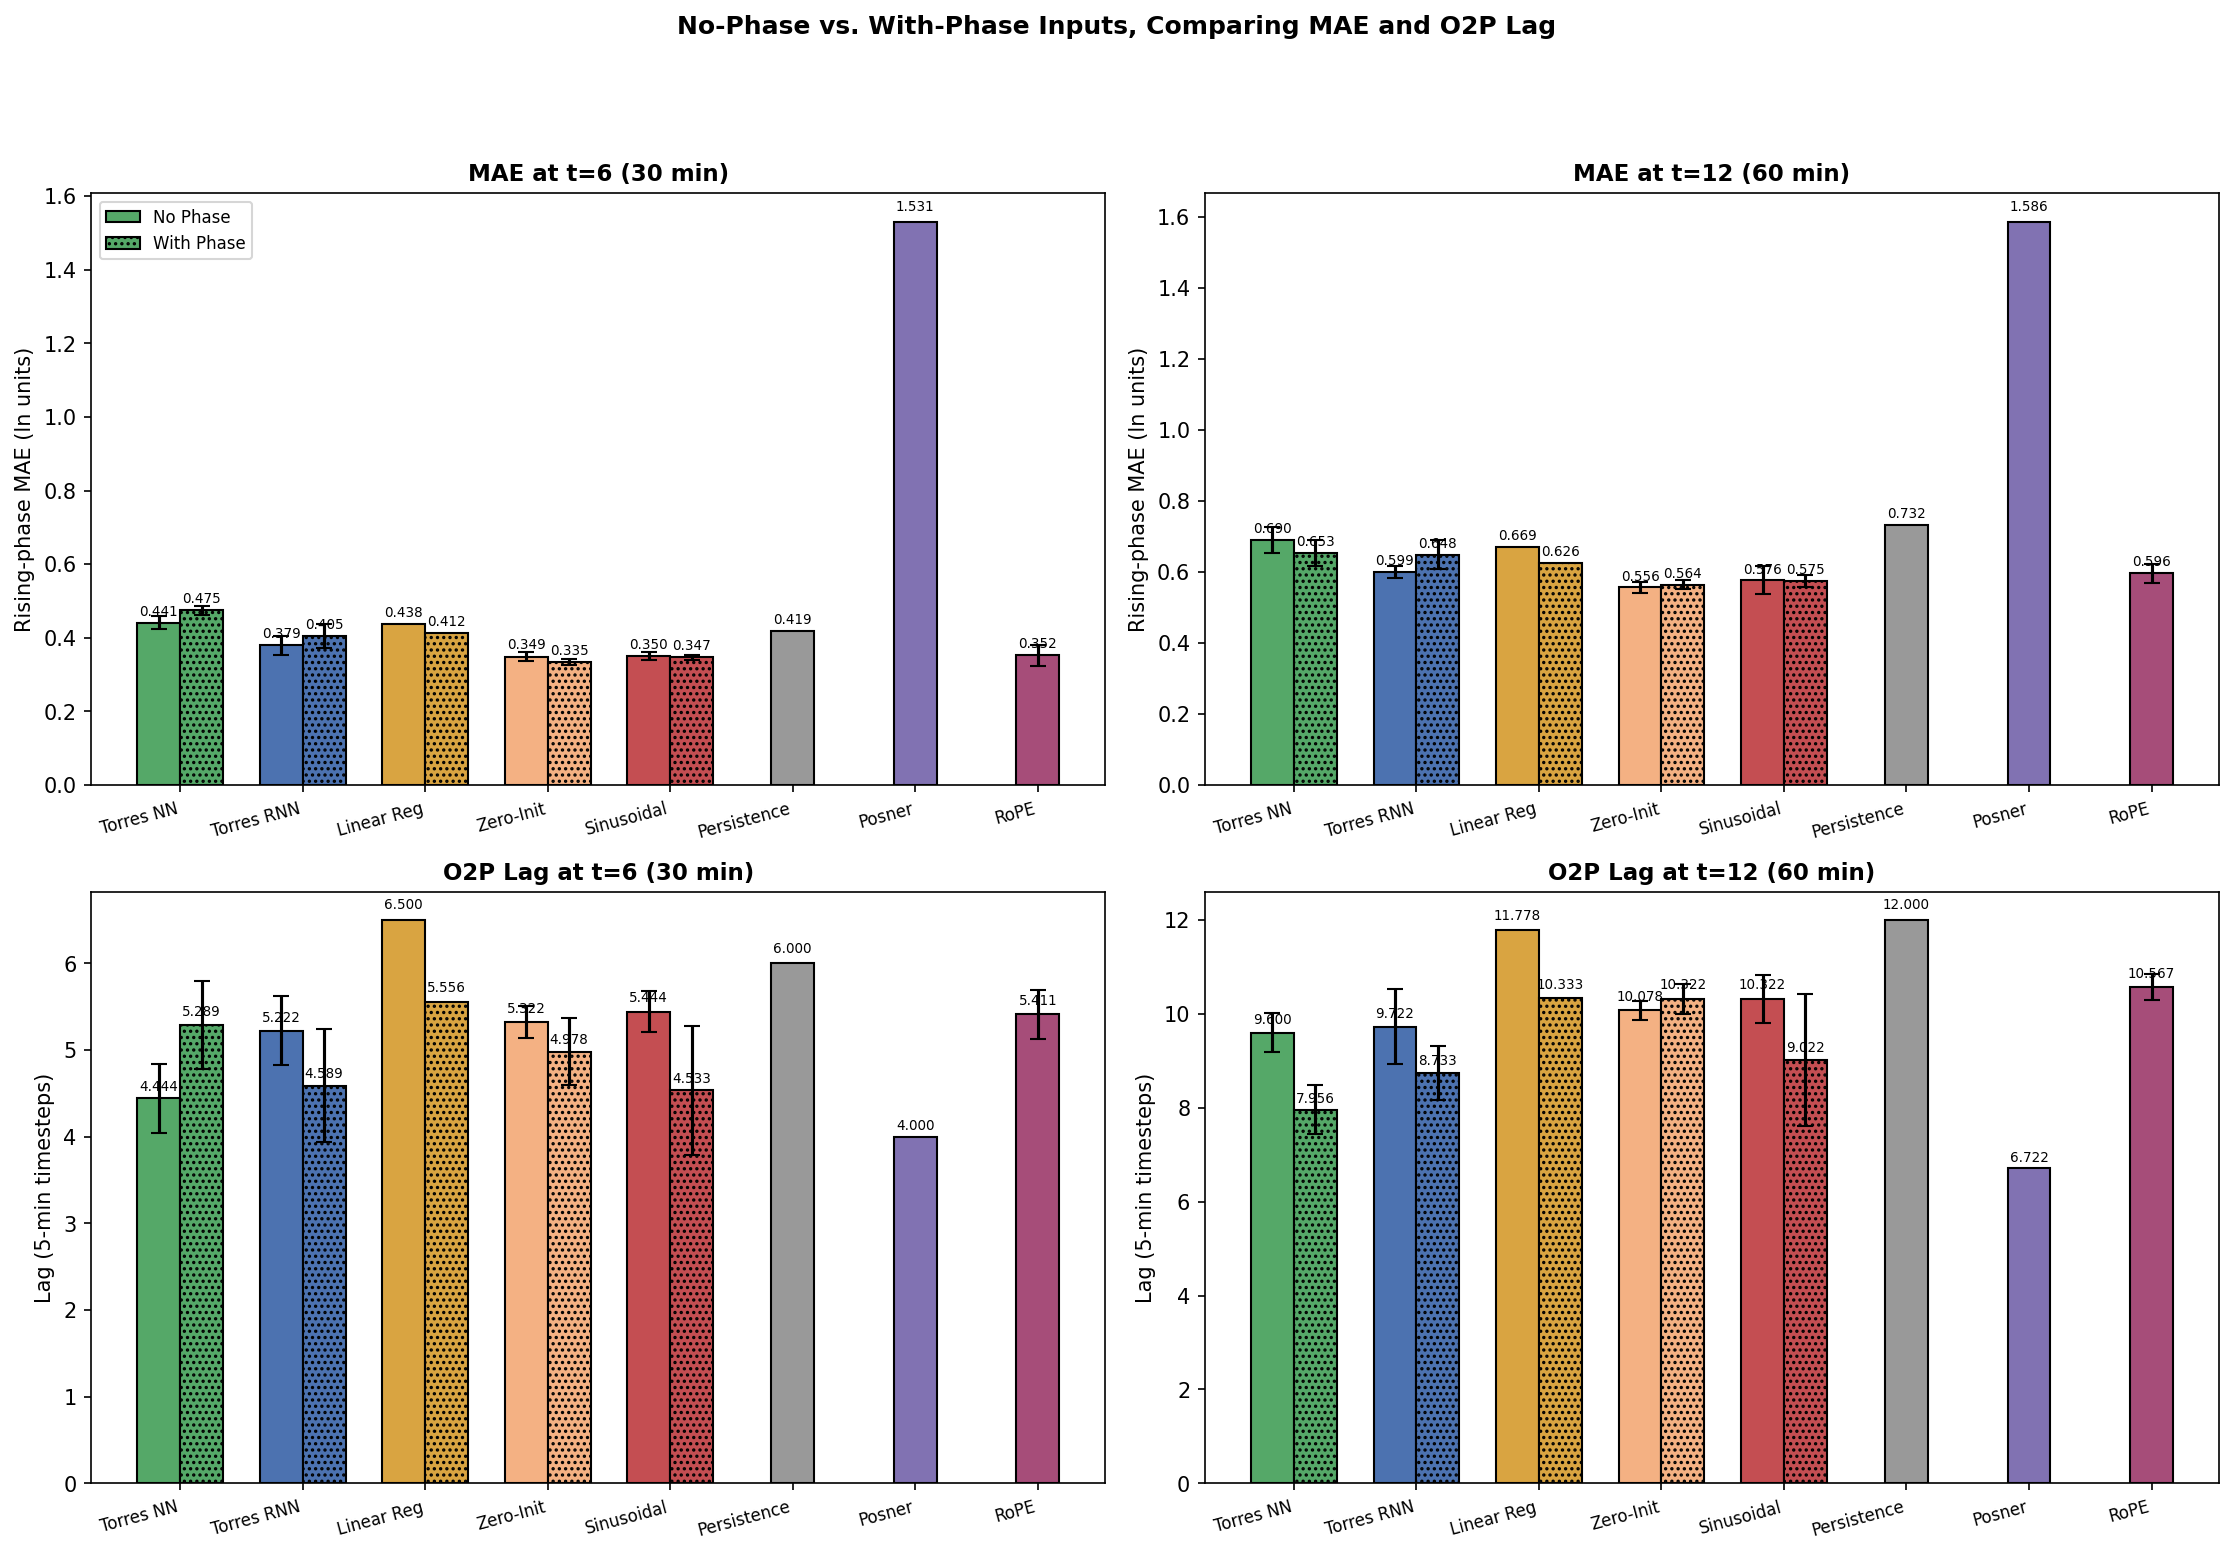
\includegraphics[width=1\textwidth]{plots/mae_lag_phase_comparison.png} % Inserts and resizes image
    \caption{Comparison of MAE and Lag compared to other models} 
    \label{fig: Comparison of lag and MAE between Torres and transformer models} % Label used for referencing
\end{figure}

% \hl{add phases lag and MAE. possibly table. get rid of chart title}


Additional evaluations are needed to score our proton intensity predictions. We evaluate our ability to predict protons $>10 \text{ MeV}$ above $10 \text{ pfu}$ (Threshold to Peak). a warning period is defined  as all consecutive timestamps during which the prediction is above the threshold.

\begin{table}[H]
\centering

\label{tab:f1_comparison}
\resizebox{\textwidth}{!}{%
\begin{tabular}{l cccc cccc}
\toprule
& \multicolumn{4}{c}{$t+6$} & \multicolumn{4}{c}{$t+12$} \\
\cmidrule(lr){2-5} \cmidrule(lr){6-9}
Method & W & EW & AW & EAW & W & EW & AW & EAW \\
\midrule
Linear Reg   & 0.000 & 0.000 & 0.160 & 0.160 & 0.100 & 0.100 & 0.519 & 0.519 \\
Zero-Init    & \textbf{0.040} (0.055) & \textbf{0.040} (0.055) & 0.613 (0.078) & 0.613 (0.078) & 0.132 (0.079) & \textbf{0.150} (0.120) & 0.732 (0.075) & 0.716 (0.045) \\
Sinusoidal   & 0.038 (0.052) & 0.039 (0.053) & 0.632 (0.068) & 0.632 (0.068) & \textbf{0.137} (0.053) & 0.137 (0.053) & \textbf{0.745} (0.091) & \textbf{0.745} (0.091) \\
RoPE         & 0.036 (0.081) & 0.036 (0.081) & \textbf{0.643} (0.112) & \textbf{0.643} (0.112) & 0.115 (0.079) & 0.115 (0.079) & 0.690 (0.071) & 0.690 (0.071) \\
\bottomrule
\end{tabular}%
}

\caption{Event-detection F1 scores by approach and encoding method, 2-hour alert window (mean $\pm$ std over 5 seeds; Linear Regression is a single deterministic run) No-Phases.}
\end{table}
\begin{table}[H]
\centering

\label{tab:f1_comparison}
\resizebox{\textwidth}{!}{%
\begin{tabular}{l cccc cccc}
\toprule
& \multicolumn{4}{c}{$t+6$} & \multicolumn{4}{c}{$t+12$} \\
\cmidrule(lr){2-5} \cmidrule(lr){6-9}
Method & W & EW & AW & EAW & W & EW & AW & EAW \\
\midrule
Linear Reg   & 0.348 & 0.364 & 0.562 & 0.581 & 0.250 & 0.261 & 0.706 & 0.788 \\
Torres M1    & 0.30 & 0.48 & 0.62 & 0.76 & 0.16 & \textbf{0.38} & 0.72 & 0.85 \\
Posner       & \textbf{0.56} & \textbf{0.69} & 0.59 & 0.67 & \textbf{0.31} & 0.36 & 0.67 & 0.72 \\
Zero-Init    & 0.309 (0.092) & 0.320 (0.091) & 0.743 (0.055) & 0.761 (0.063) & 0.176 (0.054) & 0.206 (0.040) & 0.782 (0.039) & 0.821 (0.042) \\
Sinusoidal   & 0.350 (0.099) & 0.365 (0.102) & \textbf{0.806} (0.067) & \textbf{0.829} (0.068) & 0.226 (0.043) & 0.238 (0.043) & \textbf{0.824} (0.024) & \textbf{0.852} (0.025) \\
\bottomrule
\end{tabular}%
}

\caption{Event-detection F1 scores by approach and encoding method, 2-hour alert window (mean $\pm$ std over 5 seeds; Linear Regression, Torres M1, and POSNER are single deterministic runs), Phases.}
\end{table}









